\documentclass[10pt]{article}
\usepackage[utf8]{inputenc}
\usepackage[margin=1in]{geometry}
\usepackage{amsmath}
\usepackage{amssymb}
\usepackage{graphicx}
\usepackage{hyperref}
\usepackage{cite}
\usepackage{caption}

\title{\vspace{-3cm}CS 474 Project Report}
\author{Brock Gregersen}
\date{\vspace{-0.25cm}\today}

\begin{document}

\maketitle

\vspace{-1.5cm}
\section{Background}
In many scientific and engineering applications, it is desired to know the global temperature distribution of a system, however, only a limited number of temperature measurements are available. This project explores the use of Physics-Informed Neural Networks (PINNs) to solve the inverse heat equation problem for a flat plate. This project explores square plates and plates of arbitrary shape defined by a signed distance function (SDF). It also explores two different types of boundary conditions: constant temperature and constant flux. The goal is to train a PINN to predict the temperature distribution across the plate given a limited number of temperature measurements and the governing physics of heat conduction.

\section{Dataset}
The dataset consists of temperature measurements taken from a sparse set of points on the plate. In reality, these measurements could be obtained from thermocouples placed at specific locations. For this project, datasets are generated using numerical simulations of the heat equation under various conditions, including different plate geometries, boundary conditions, and noise levels. Each dataset includes the spatial and temporal coordinates of the measurement points, and the corresponding temperature values. Figures~\ref{fig:fig1} and \ref{fig:fig2} shows an example of sparse temperature measurements used the reconstructed temperature field.

\begin{figure}[ht]
    \begin{minipage}{0.35\textwidth}
        \centering
        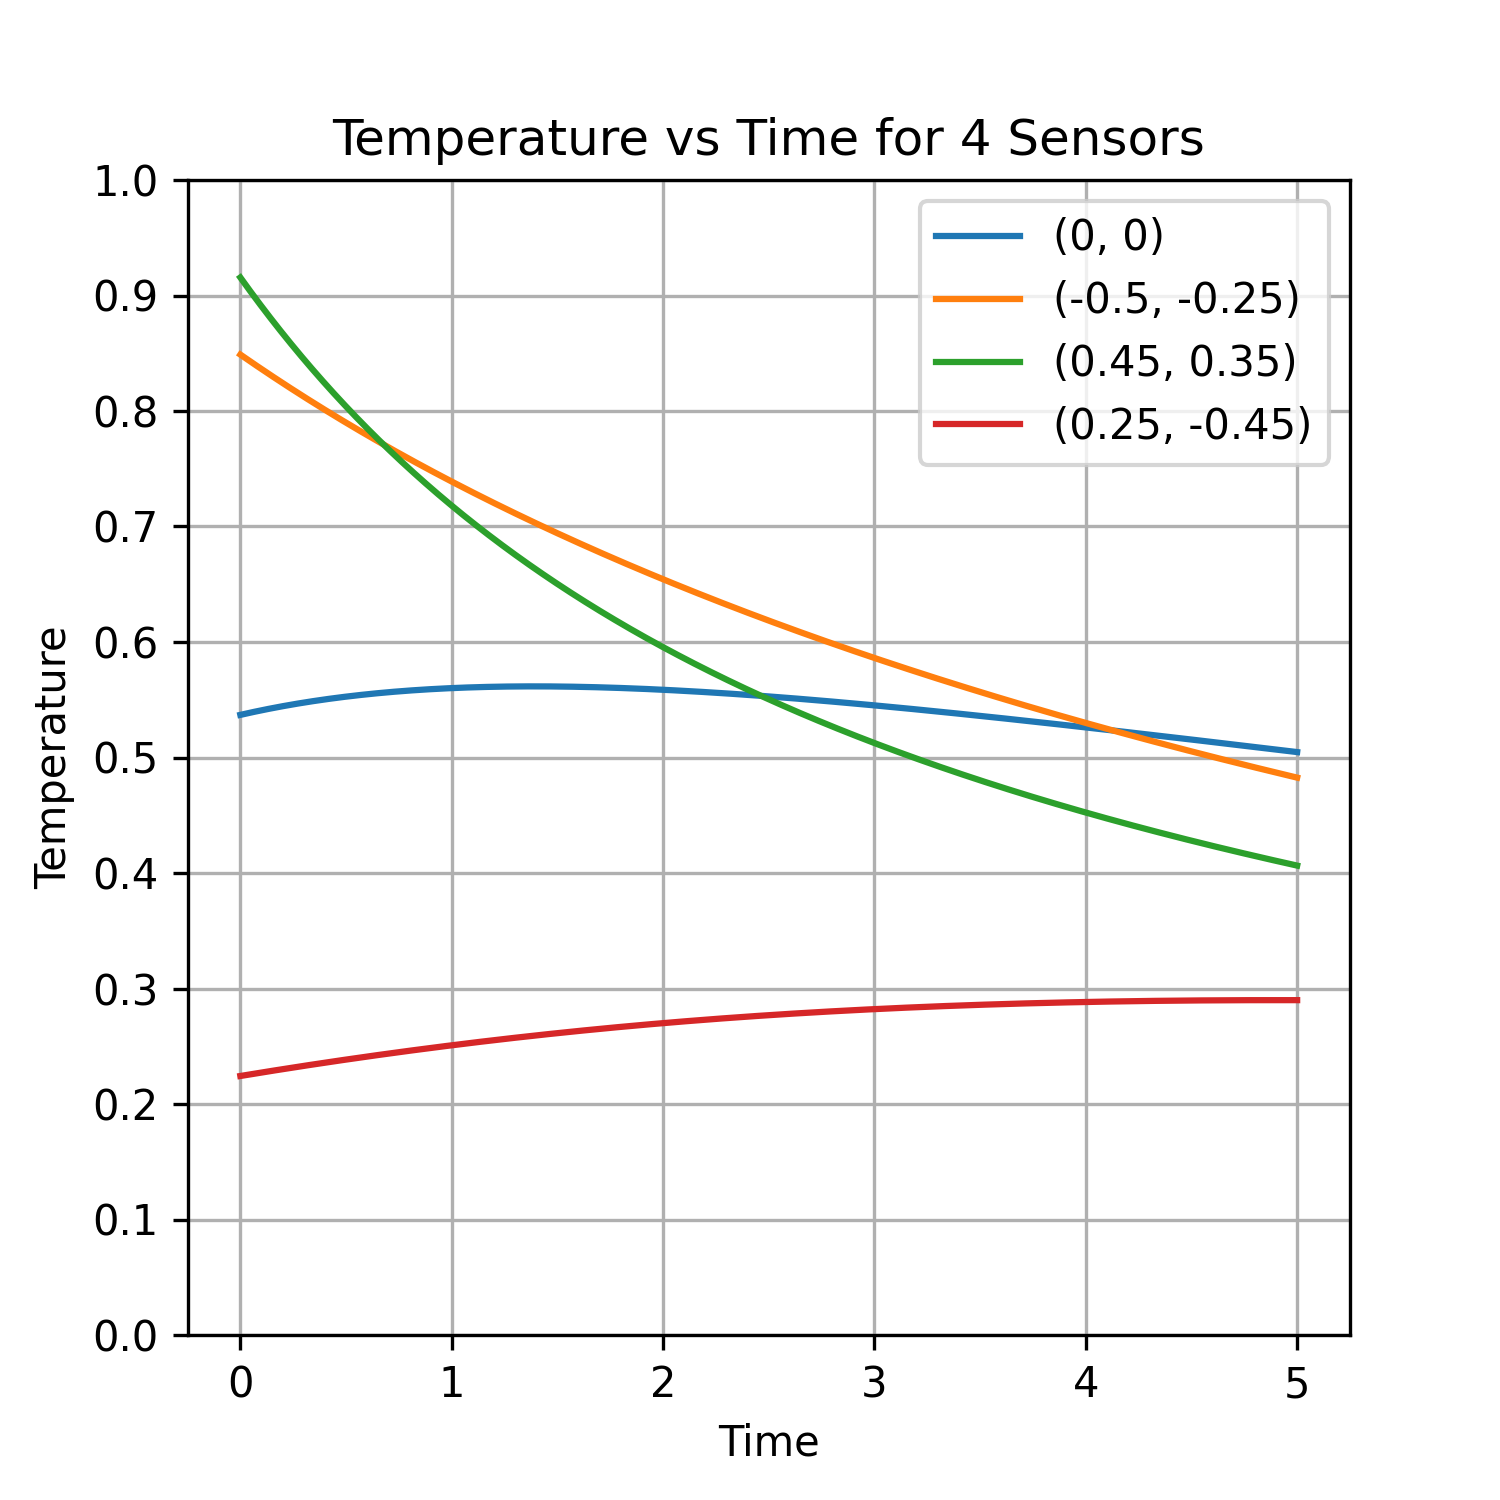
\includegraphics[width=\textwidth]{plots/dual_gaussian_4.png}
        \captionof{figure}{Temperature data from 4 thermocouples.}
        \label{fig:fig1}
    \end{minipage}
    \hfill
    \begin{minipage}{0.6\textwidth}
        \centering
        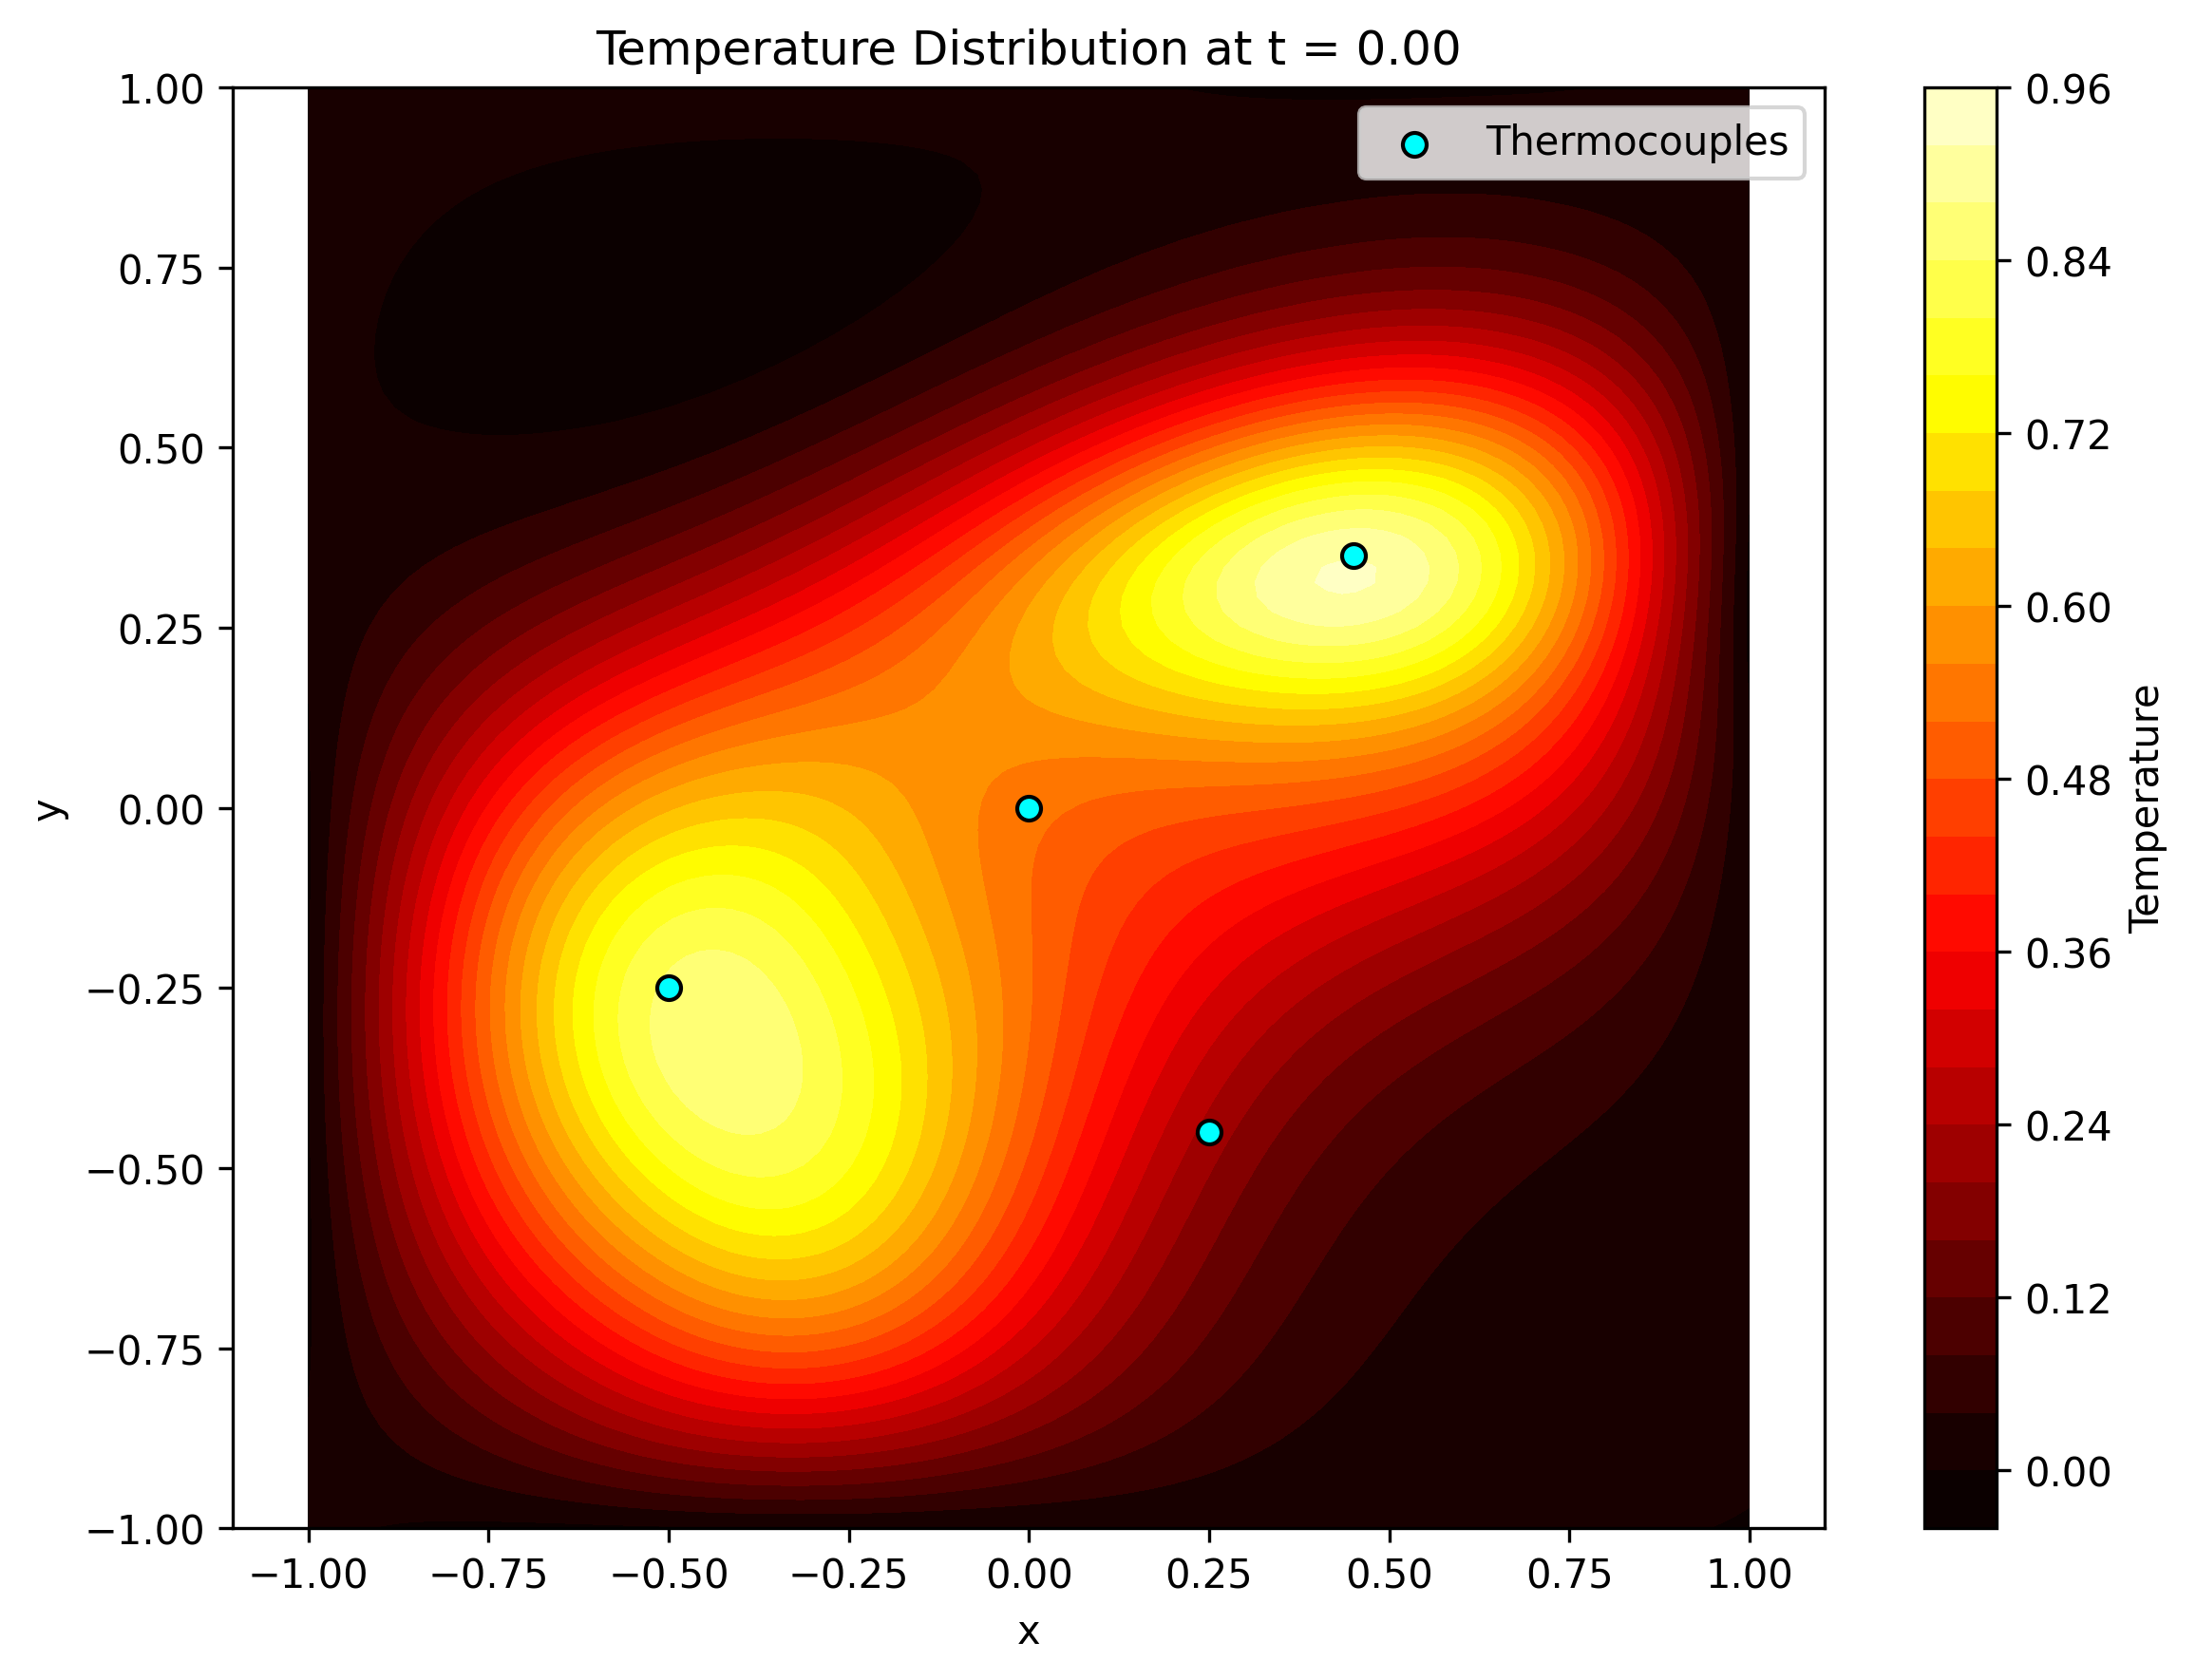
\includegraphics[width=\textwidth]{plots/dual_gaussian_output.png}
        \captionof{figure}{Reconstructed temperature field at one time step.}
        \label{fig:fig2}
    \end{minipage}
\end{figure}

\section{Approach}
\subsection{Model Architecture}
The PINN architecture consists of a fully connected feedforward neural network that takes coordinates (x, y, t) as input and outputs the predicted temperature (T). We use a network with 3 hidden layers of 64 neurons each. A SiLU activation function is used so that a 2nd derivative can be calculated as needed for the loss functions.

\subsection{Loss Functions}
The loss function for training the PINN consists of three components:
\subsubsection{Data Loss}
This term measures the mean squared error between the predicted temperatures and the observed temperatures at the measurement points from the sparse dataset:
\[L_{\text{data}} = \frac{1}{N} \sum_{i=1}^{N} (T_{\text{pred}}(x_i, y_i, t_i) - T_{\text{obs}}(x_i, y_i, t_i))^2\]

\subsubsection{Physics Loss}
This term enforces the governing physics of heat conduction by penalizing deviations from the heat equation at a randomly sampled set of points in the domain:
\[L_{\text{physics}} = \frac{1}{M} \sum_{j=1}^{M} \left( \frac{\partial T_{\text{pred}}}{\partial t}(x_j, y_j, t_j) - \alpha \left( \frac{\partial^2 T_{\text{pred}}}{\partial x^2}(x_j, y_j, t_j) + \frac{\partial^2 T_{\text{pred}}}{\partial y^2}(x_j, y_j, t_j) \right) \right)^2\]
where \(\alpha\) is the thermal diffusivity of the material.
\subsubsection{Boundary Loss}
This term enforces boundary conditions at randomly sampled boundary points. For constant temperature and constant flux conditions respectively, the loss is defined as:
\[
\begin{aligned}
L_{\text{boundary}} &= \frac{1}{P}\sum_{k=1}^{P}\left(T_{\text{pred}}(x_k,y_k,t_k)-T_{\text{boundary}}\right)^2
\qquad
L_{\text{boundary}} &= \frac{1}{P}\sum_{k=1}^{P}\left(\frac{\partial T_{\text{pred}}}{\partial n}(x_k,y_k,t_k)-q_{\text{boundary}}\right)^2
\end{aligned}
\]
where \(q_{\text{boundary}}\) is the prescribed normal temperature gradient (heat flux).
\subsection{Training Procedure}
The PINN is trained using an Adam optimizer to minimize the combined loss function:
\[L = L_{\text{data}} + L_{\text{physics}} + L_{\text{boundary}}\]
For most experiments, the model was trained for 50-100 epochs with a learning rate of 0.001. 

\section{Results}
The model was evaluated on a separate validation set of temperature measurements at locations not included in the training data. A percentage L2 error metric was used to quantify the accuracy of the predictions. Results for a selcection various configurations of boundary conditions, and noise levels, and initial conditions are presented in the following table:
\begin{table}[ht]
\centering
\begin{tabular}{|c|c|c|c|c|}
\hline
\shortstack{\textbf{Boundary}\\\textbf{Conditions}} &
\shortstack{\textbf{Initial}\\\textbf{Conditions}} &
\shortstack{\textbf{\# Measurement}\\\textbf{Locations}} &
\shortstack{\textbf{Noise}\\\textbf{Level}} &
\shortstack{\textbf{L2 Error}\\\textbf{(\%)}} \\
\hline
Constant Temperature & 1 Gaussian & 8 & 0\% & 1.67\% \\
Constant Temperature & 2 Gaussians & 4 & 0\% & 10.87\% \\
Constant Temperature & 2 Gaussians & 8 & 0\% & 7.46\% \\
Constant Temperature & 2 Gaussians & 8 & 10\% & 11.25\% \\
Insulated & 2 Gaussians & 8 & 0\% & 22.75\% \\
\hline
\end{tabular}
\caption{L2 error percentages for different configurations of plate geometry, boundary conditions, and noise
levels.}
\end{table}

\newpage

\section{Time Log}
\begin{table}[ht]
\centering
\begin{tabular}{|c|l|c|}
\hline
\textbf{Date} & \textbf{Summary} & \textbf{Hours Spent} \\
\hline
2026-02-19 & Forward simulation for dataset creation & 1 \\
2026-02-24 & Finished basic forward sim & 1 \\
2026-03-04 & Set up PINN architecture and dataloader & 1 \\
2026-03-16 & Loss functions & 1 \\
2026-03-17 & Training loop & 1.5 \\
2026-03-20 & Updated training loop, made some architecture & 2 \\
& and hyperparameter changes & \\
2026-03-27 & Parameter scheduling, gradient clipping, other debug & 2 \\
2026-03-28 & Improved forward sim data export, & 1.5 \\
& added weight export to training loop & \\
2026-03-30 & Researched activation functions, tested with basic dataset & 2 \\
2026-03-31 & Critical dataset bug fix, added dynamic loss weighting & 1.5 \\
2026-04-04 & Added parameterized thermal diffusivity & 1 \\
2026-04-06 & Implemented SDF based geometry & 2 \\
2026-04-15 & Reworked forward sim and loss functions & 2 \\
& for constant flux boundary conditions & \\
2026-04-16 & Constant flux BCs for arbitrary geometry & 2 \\
2026-04-17 & Finished constant flux BCs, added validation & 2 \\
2026-04-18 & Mathematically defined loss functions, & 2 \\
&  started compiling results & \\
2026-04-19 & Finished compiling results, finalized report & 1 \\

\hline
\textbf{Total} & & \textbf{26.5} \\
\hline
\end{tabular}
\caption{Time log for project tasks.}
\end{table}

\end{document}